%3.1. pi-SoD-M metamodels (presentar los metamodels)


The {\em A-policy} based services' composition meta-model (see  in Figure \ref{fig:servicecompositionmodel})
represents  a workflow needed to implement a services' composition, identifying those entities that collaborate in the business processes (called {\sc Business Collaborators} \footnote{We use {\sc capitals} for referring to meta-models' classes.}) and the {\sc Actions} that  they perform. This model is represented by means of a UML activity diagram. Thus, as shown in Figure \ref{fig:e-scomposition-metamodel}, the meta-model includes typical modeling elements of the activity diagram such as {\sc ActivityNodes}, {\sc InitialNodes} and {\sc FinalNodes}, {\sc DecisionNodes}, etc., along with new elements defined by SOD-M such as {\sc Business Collaborators}, {\sc ServiceActivity} and {\sc Action} (see the white  elements   in Figure \ref{fig:servicecompositionmodel}).

\begin{itemize}
\item A {\sc Business Collaborator} element represents those entities that collaborate in the business processes by performing some of the required actions. They are graphically presented as a partition in the activity diagram. A collaborator can be either internal or external to the system being modelled. When the collaborator of the business is external to the system, the attribute {\sf\small IsExternal} \footnote{We use the {\sf sans serif} font for referring to models' classes defined using a meta-model.} of the collaborator is set to true.

\item {\sc Action}, a kind of {\sc ExecutableNode}, are represented in the model as an activity. Each action identified in the model describes a fundamental behaviour unit which represents some type of transformation or processing in the system being modelled. There are two types of actions: i) a WebService (attribute Type is {\sf\small WS}); and ii) a simple operation that is not supported by a Web Service, called an {\sc ActivityOperation} (attribute Type is {\sc AOP}).
    
\item The {\sc ServiceActivity} element is a composed activity that  must be carried out as part of a business service and is composed of one or more executable nodes.
\end{itemize}

 \begin{figure}[htpb]
\centering
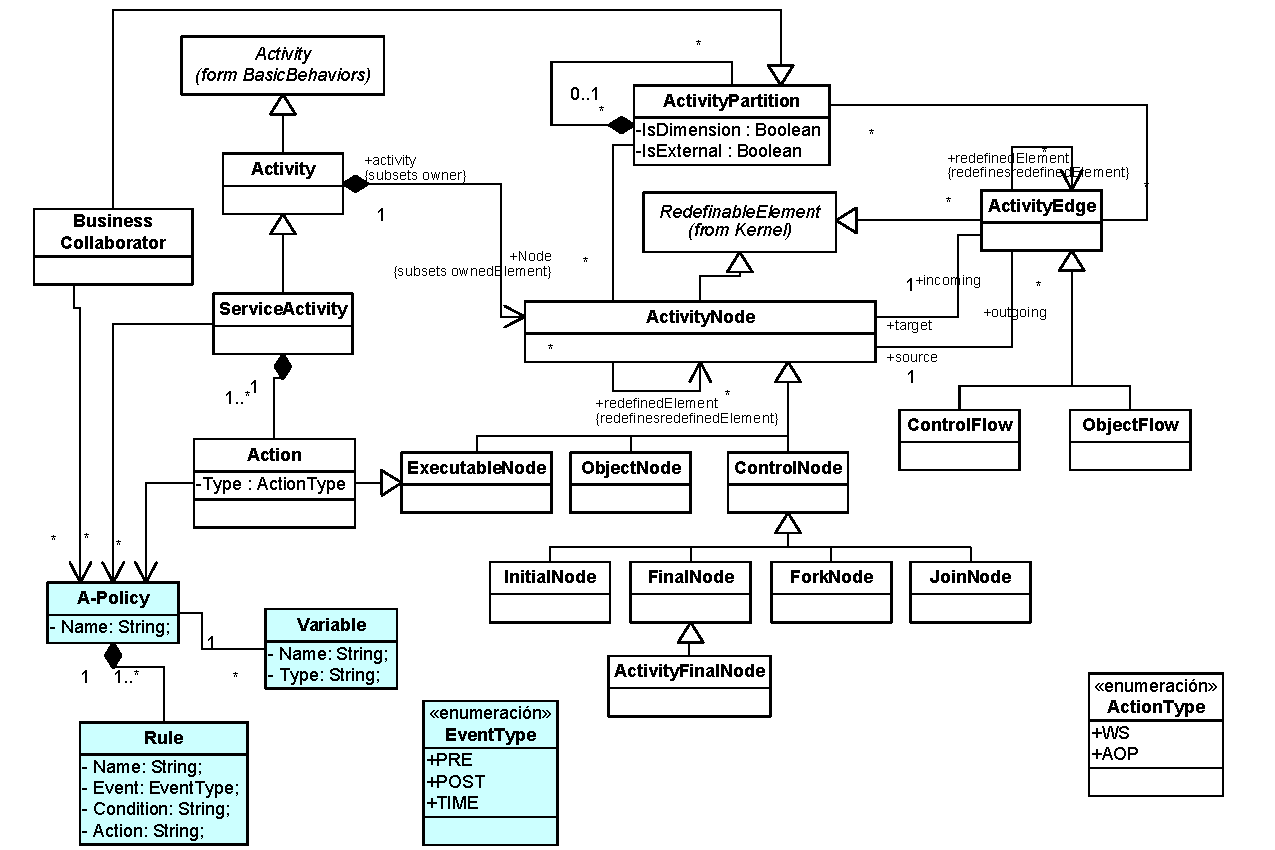
\includegraphics[width=0.80\textwidth]{figs/E-service-composition-metamodel}
\caption{{\em A-policy} based services' composition meta-model ($\pi$-SCM)}
\label{fig:e-scomposition-metamodel}
\end{figure}

To illustrate the use of the $\pi$-SCM meta-model we used it for defining the {\em A-policy} based composition model of the "To Publish Music" scenario (see
Figure \ref{fig:servicecompositionmodel}). There are three external business collaborators ({\em Spotify, Twitter} and {\em Facebook} \footnote{We use {\em italics} to refer to concrete values of the classes of a model that are derived from the classes of a meta-model.}). It also shows the business process  of the  "To Publish Music" application that consists of three service activities: {\em Listen Music}, {\em Public Music} and {\em Confirmation}. Note that  the action {\em Publish Music} of the application calls the actions of two service collaborators namely {\em Facebook} and {\em Twitter}.

Instead of programming different protocols within the application logic, we propose to include the modeling of non-functional constraints like transactional behaviour, security and adaptability  at the early stages of the services' composition engineering process. We model non-functional constraints of services' compositions using the notion of {\em A-policy} \cite{Espinosa-Oviedo2011a,CIC:eovszmc09c}, a kind of pattern for specifying {\em A-policy} types. In order to represent constraints associated to services compositions, we extended the SOD-M services' composition model with two concepts: {\sc Rule} and {\sc A-policy} (see blue elements in the $\pi$-SCM meta-model in Figure \ref{fig:e-scomposition-metamodel}).

The {\sc Rule} element represents an event - condition - action rule where the {\sc Event} part represents the moment in which a constraint  can be evaluated according to a condition represented by the {\sc Condition} part and the  action  to be executed for reinforcing  it represented by the {\sc Action} part. 
%An {\em A-policy}  describes  specific constraint types that can correspond to non-functional constraints like  transactional behaviour, security and adaptability. 
%An {\em A-policy}  defines a set of constraints over the execution states of the servicesÕ composition and defines strategies to enforce this property at the servicesÕ composition execution time.
An {\em A-policy} groups a set of rules. It describes global variables and operations that can be shared by the rules and that can be used for expressing their Event  and Condition parts. An {\em A-Policy} is associated to the elements {\sc BusinessCollaborator}, {\sc ServiceActivity} and, {\sc Action}  of the $\pi$-SCM meta-model (see Figure \ref{fig:e-scomposition-metamodel}) . 

\begin{figure}[htpb]
\centering
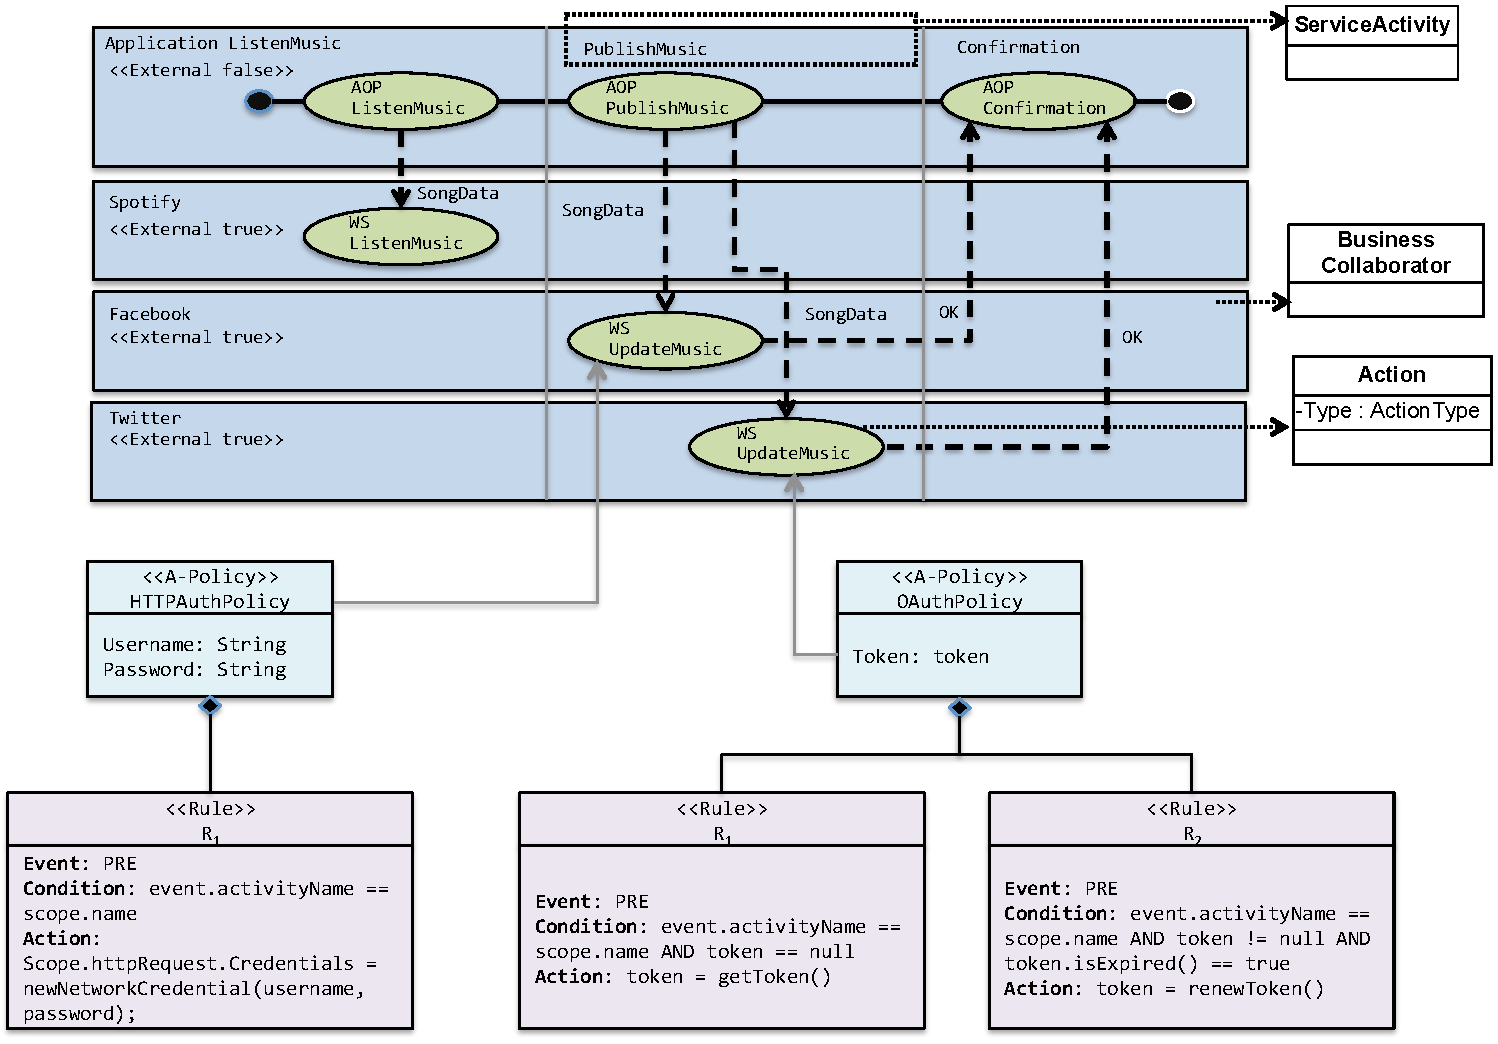
\includegraphics[width=0.70\textwidth]{figs/e-composition-model}
\caption{Services' composition model for the business service "To publish music"}
\label{fig:servicecompositionmodel}
\end{figure}

Given that {\em Facebook} and {\em Twitter} services require authentication protocols in order to execute methods that will read and update the users' space. A call to such services must be part of the authentication protocol required by these services.
In the example we  associate two authentication policies, one for the open authentication protocol, represented by the class {\sf\small Twitter OAuthPolicy} that will be associated to the activity  {\sf\small UpdateTwitter} (see Figure \ref{fig:servicecompositionmodel}). In the same way, the  class {\sf\small Facebook HTTPAuthPolicy}, for the http authentication protocol will be associated to the activity {\sf\small UpdateFacebook}.
 {\sf\small OAuth}  implements the open authentication protocol.
As shown in Figure \ref{fig:servicecompositionmodel}, the {\em A-policy} has a variable {\sf\small Token} that will be used to store the authentication token provided by the service. This variable type is imported through the library {\sf\small OAuth.Token}. The {\em A-policy}  defines two rules, both can be triggered by events of type {\sf\small ActivityPrepared}: (i) if no token has been associated to the variable {\sf\small token}, stated in by the condition of rule {\sf\small R$_1$}, then a token is obtained (action part of {\sf\small R$_1$}); (ii) if the token has expired, stated in the condition of rule {\sf\small R$_2$}, then it is renewed (action part of {\sf\small R$_2$}). Note that the code in the actions profits from the imported  {\sf\small OAuth.Token} for transparently obtaining or renewing a token from a third party.

{\sf\small HTTP-Auth} implements the HTTP-Auth protocol.  As shown in Figure  \ref{fig:servicecompositionmodel}, the {\em A-policy} imports an http protocol library and it has two variables {\sf\small username} and {\sf\small password}.  The event of type {\sf\small ActivityPrepared} is the triggering event of the rule {\sf\small R$_1$}. On the notification of an event of that type, a credential is obtained using the username and password values. The object storing the credential is associated to the scope, i.e., the activity that will then use it for executing the method call.

Thanks to rules and policies  it is possible to model and associate non-functional properties to services' compositions  and then generate the code. For example, the atomic integration of information retrieved from different social network services, automatic generation of an integrated view of the operations executed in different social networks or for providing security in the communication channel when the payment service is called.

Back to the  definition process of a SIS, once the {\em A-policy} based services' composition model has been defined, then it can be transformed into a model (i.e., $\pi$-PEWS model) that can support then executable code generation. The following Section describes the $\pi$-PEWS  meta-model that supports this representation. 


%..--..--..--..--..--..--..--..--..--..--..--..--..--..--..--..--..--..--..--..--..--..--..--..--..--..--..--..--..--..--..--..--..--..--..--..--..--..--
\subsubsection{$\pi$-{\sc Pews}  meta-model}\label{sec:pewsmetamodel}
%..--..--..--..--..--..--..--..--..--..--..--..--..--..--..--..--..--..--..--..--..--..--..--..--..--..--..--..--..--..--..--..--..--..--..--..--..--..--
The idea of the $\pi$-{\sc Pews} meta-model is based on the services' composition approach provided by the language PEWS\cite{BaAM06,Placido2010LTPD} (\textit{Path Expressions for Web Services}), a programming language that lets the service designer  combine the methods or subprograms that
implement each operation of a service, in order to achieve the desired application logic. Figure \ref{fig:metamodel} presents the $\pi$-{\sc Pews} meta-model
consisting of  classes representing:
\begin{itemize}
\item A services' composition: {\sc Namespace} representing the interface exported by a service, {\sc Operation} that represents a call to a service method, {\sc CompositeOperation}, and  {\sc Operator} for representing a services' composition and {\sc Path} representing a services' composition.
A {\sc Path} can be an {\sc Operation} or a {\sc Compound Operation}
denoted by an identifier. A {\sc Compound Operation} is defined using an  {\sc Operator}  that can be represent  sequential ($\ . \ $) and parallel ($\ \| \ $) composition of services,
 choice ($\ + \ $) among services,
the sequential ($*$) and parallel ($\{\dots\}$) repetition of an operation or the conditional execution of an operation ($[C]S$).

\item {\em A-Policies} that can be associated to a services' composition:  {\sc A-Policy}, {\sc Rule}, {\sc Event}, {\sc Condition}, {\sc Action}, {\sc State}, and {\sc Scope}.
\end{itemize}
%
\begin{figure}
\centering
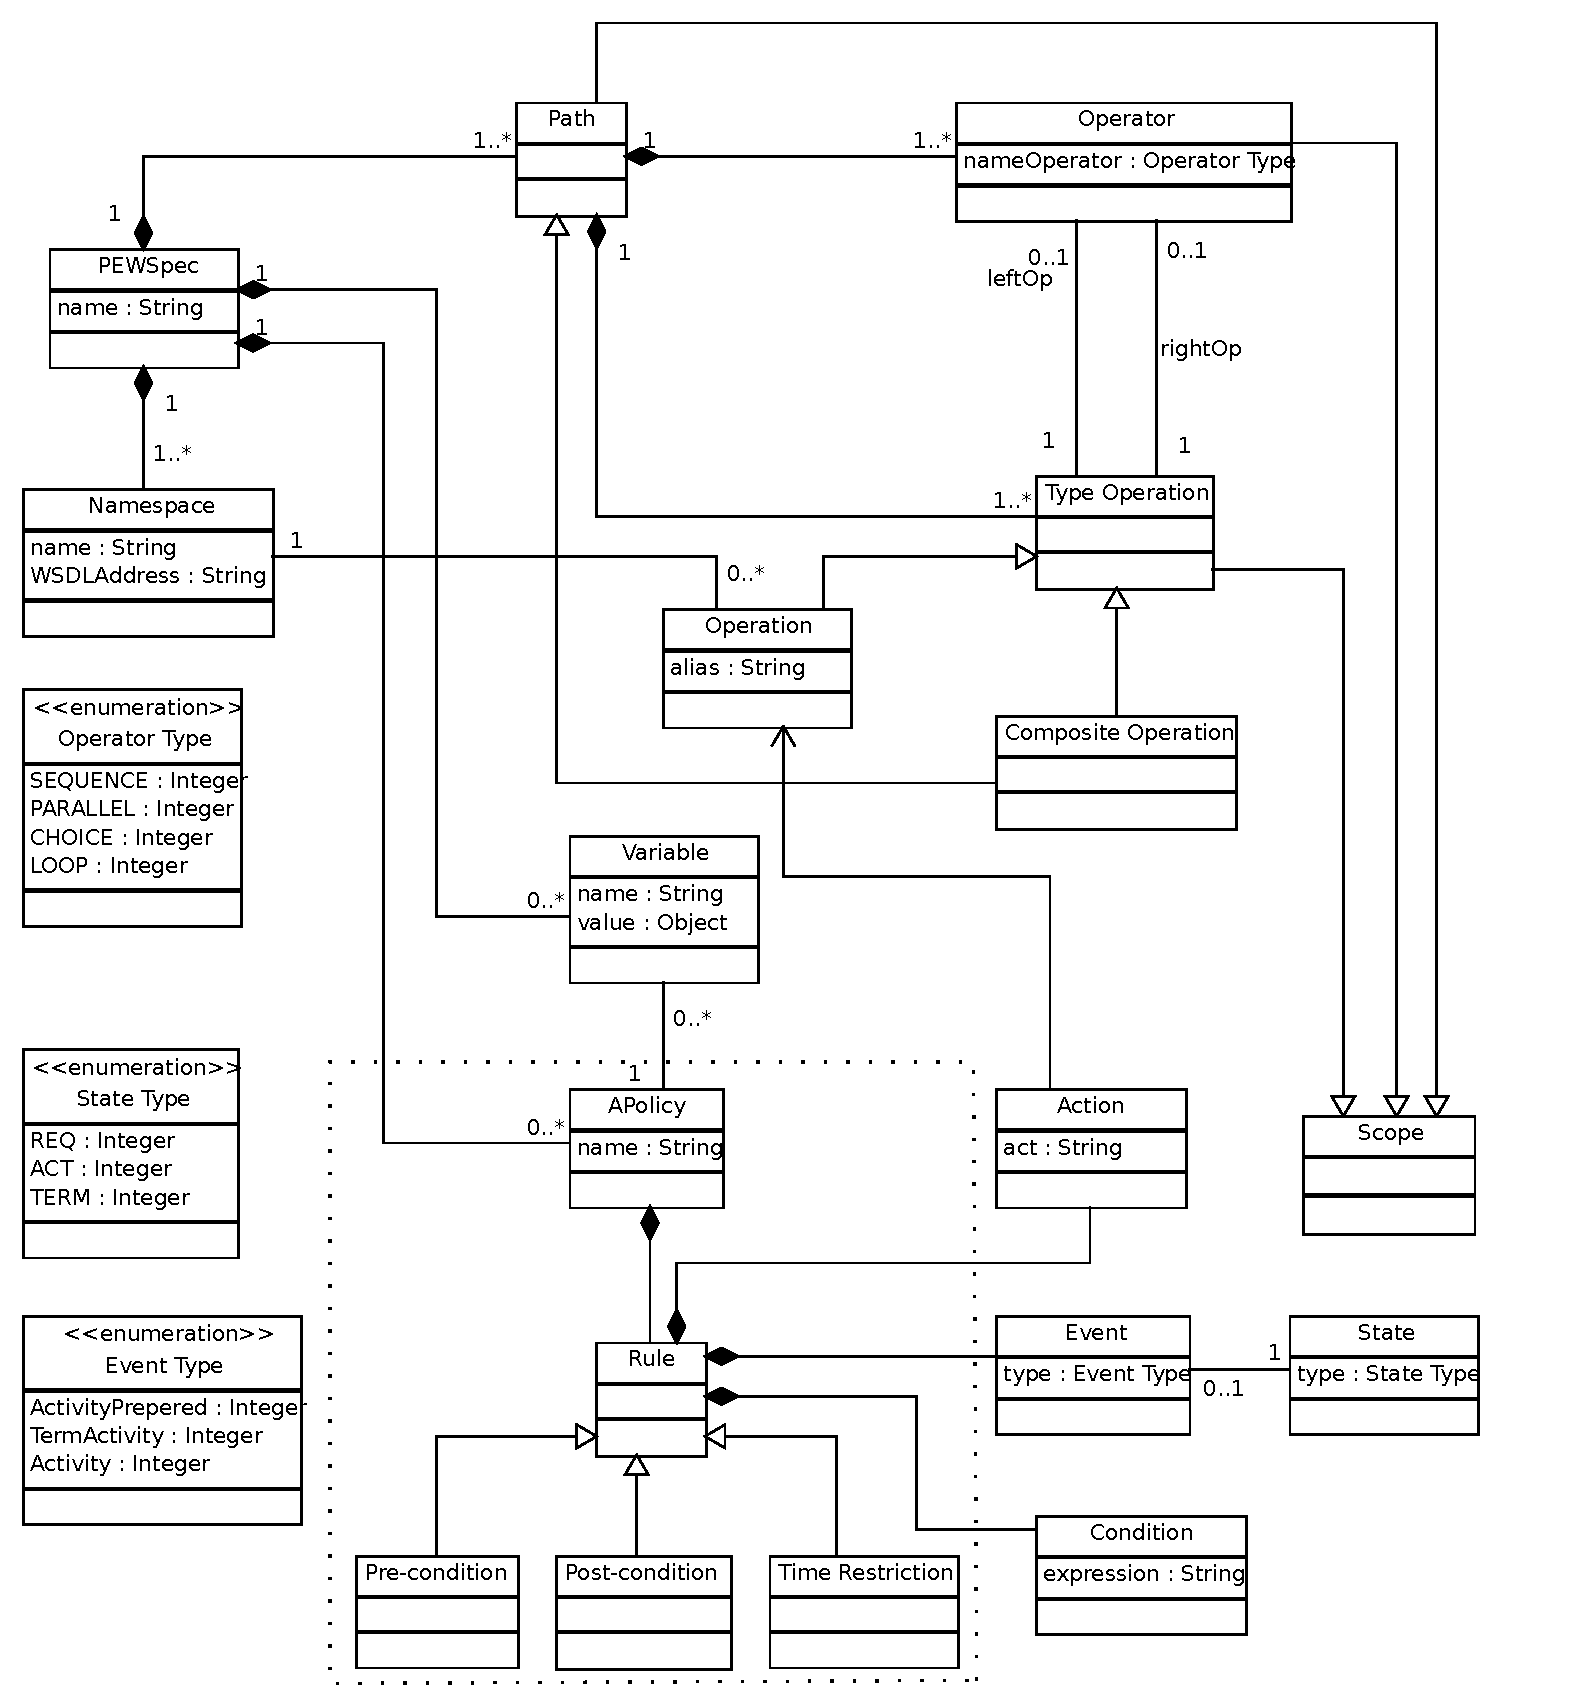
\includegraphics[width=0.80\textwidth]{figs/PEWSMetamodel}
\caption{$\pi$-{\sc Pews} Metamodel}
\label{fig:metamodel}
\end{figure}

As shown in the diagram an {\sc A-Policy} is applied to a {\sc Scope} that can be either an {\sc Operation} (e.g., an authentication protocol associated to a method exported by a service),  an {\sc Operator} (e.g., a temporal constraint associated to a sequence of operators, the authorized delay between reading a song title in Spotify and updating the walls must be less then 30 seconds), and a {\sc Path} (e.g., executing the walls' update under a strict atomicity protocol -- all or noting).  It groups a set of ECA rules, each rule having a classic semantics, i.e, {\em when an event of type E occurs if  condition C is verified then execute the action A}.  Thus, an {\em A-policy} represents a set of reactions to be possibly executed if one or several triggering events of its rules are notified.
\begin{itemize}
\item The class {\sc Scope} represents any element of a services' composition (i.e., operation, operator, path).
\item The class {\sc A-Policy} represents a recovery strategy implemented by ECA rules of the form {\sc Event} - {\sc Condition} - {\sc Action}. A {\em A-policy} has variables that represent the view of the execution state of its associated scope, that is required for executing the rules. The value of a variable is represented using the type {\sc Variable}. The class {\sc A-Policy} is specialized for defining specific constraints, for instance authentication {\em A-policies}.
\end{itemize}

%An authentication {\em A-policy} represents the situation where an invocation in
%an activity occurs until its sender and/or its recipient have been
%identified. Typically, authentication A-Policies ensure that the invocation of the activity will be done within an authentication protocol.
%

Given a $\pi$-SCM model of a specific services' based application (expressed according to the $\pi$-SCM meta-model), it is possible to generate its corresponding $\pi$-{\sc Pews} model thanks to transformation rules. The following Section describes the transformation rules between the $\pi$-SCM and $\pi$-{\sc Pews} meta-models of our method.



